\documentclass[11pt]{article}
\usepackage{titlesec}

\usepackage{titlesec}

\titleformat{\section}
  {\centering\Large\bfseries} % Style: centered, large font, bold
  {}                          % No section number
  {0em}                       % Spacing between number and title
  {}                          % Title content (unchanged)

\titleformat{\subsection}
  {\normalfont\Large\bfseries}   % Formatting style: font, size, bold, etc.
  {}                             % Empty to suppress numbering
  {0em}                          % Spacing between label and title (ignored here)
  {}                             % Code before the title

\renewcommand{\abstractname}{\Large Abstract} % Change title size (if required)
\renewenvironment{abstract}
  {\begin{center}\bfseries\Large Abstract\vspace{1em}\end{center}%
   \normalsize} % Adjust text size here
  {}

\usepackage{amsmath, amssymb}
\usepackage{xcolor}
\usepackage{enumerate}
\usepackage{graphicx}
\usepackage{tabularx}
\usepackage{algorithm}
\usepackage{algpseudocode}
\usepackage{tikz}
\usepackage{tikz-qtree}
\usepackage{subcaption}

\usepackage{natbib}  % For bibliography
\usepackage{hyperref}  % For clickable links

\usepackage{indentfirst}

%
% Basic Document Settings
%  

\topmargin=-0.45in
\evensidemargin=0in
\oddsidemargin=0in
\textwidth=6.5in
\textheight=9.0in
\headsep=0.25in

\linespread{1.1}

\usepackage{setspace}
\usepackage{listings}
\lstset{
  language=Python,                   % Set programming language
  keywordstyle=\bfseries\color{blue},% Bold keywords in blue
  stringstyle=\color{teal},          % Strings in teal
  commentstyle=\itshape\color{red}, % Italicize comments in gray
  frame=lines,                       % Add lines at the top and bottom
  rulecolor=\color{gray!30},         % Light gray for the frame
  tabsize=4,                         % Set tab size to 4 spaces
  captionpos=b,                      % Place caption below the code
  emphstyle=\bfseries\color{purple}, % Highlight emphasized text
  escapeinside={(*@}{@*)},           % Allows for LaTeX inside code
  extendedchars=true                 % Support extended characters
}



% headers, footers, titles
\newcommand{\CourseName}{SI140A Probability and Statistics Final Project}
\newcommand{\DueDate}{2025/1/12 10:59pm}


\title{
    \vspace{100pt}
    \bigskip
    \textbf{\CourseName:} \\
    \textbf{Performance Evaluation of Bandit Learning Algorithms} \\
    \bigskip
}
\author{Jingran Fan \and Anrui Wang \and Zhao Lu}
\bigskip
\date{Due date: \DueDate}

\begin{document}
\setlength{\parindent}{2em}

\maketitle

\newpage

\begin{abstract}

Multi-armed bandit problems are fundamental models in sequential decision-making under uncertainty, wherein an agent must choose from several options (arms) over repeated trials to maximize cumulative rewards. These problems capture the delicate balance between exploration—seeking information about less-known options—and exploitation—leveraging current knowledge to select the best option. Classical bandit learning algorithms, such as 
$\epsilon$-greedy, Upper Confidence Bound (UCB), and Thompson Sampling (TS), have been extensively studied and form the cornerstone of modern reinforcement learning techniques. More recently, Bayesian approaches that incorporate prior beliefs and update them with observed data have gained traction, offering theoretical elegance and robust performance in a variety of settings.

This project focuses on evaluating the performance of well-known bandit algorithms through numerical experiments. In Part I, we consider classical bandit algorithms operating on Bernoulli arms with parameters provided by an oracle. Although the oracle’s parameters and optimal attainable reward (the “oracle value”) are unknown to the algorithms, they provide a ground truth reference for performance comparison. We implement and benchmark 
$\epsilon$-greedy (with various $\epsilon$-values), UCB (with different confidence scales), and TS (with varying Beta priors) under identical experimental conditions. By analyzing their regret—defined as the gap between the algorithm’s cumulative reward and the oracle value—we investigate how tuning parameters and prior knowledge impacts the exploration-exploitation trade-off.

In the optional Part II, we extend our analysis to a Bayesian bandit setting with discounted rewards, where prior distributions on arm parameters are continuously updated as more data is observed. We examine intuitive heuristics and discuss why these heuristics may fail to achieve optimality. Furthermore, we explore the derivation of optimal policies through recursive equations and investigate practical methods for exact and approximate solutions.

Overall, this project aims to provide a rigorous empirical evaluation of both classical and Bayesian bandit algorithms. By comparing their performance and understanding their underlying trade-offs, we gain deeper insights into bandit learning theory and develop intuition for selecting and designing effective strategies in diverse applications.
\end{abstract}

\newpage

\tableofcontents

\newpage

\newpage
\section{Introduction}

In many real-world scenarios—from online advertising to medical trials—decision-makers must choose actions to maximize cumulative rewards. However, these decisions also provide valuable information that can guide future actions. This creates a fundamental tension between exploiting what we already know to gain immediate benefits and exploring new options to potentially improve future outcomes. This challenge is central to the field of reinforcement learning and is known as the exploration-exploitation trade-off.

A classic illustration is the multi-armed bandit problem. Imagine walking into a casino and facing a slot machine with multiple arms, each offering a different, unknown payoff distribution. Your goal is to pull the arms over a sequence of trials to earn as many rewards as possible. Since you do not know which arm is best, you must try them out (exploration) while continuing to play the arm that seems most promising (exploitation). Crucially, the reward probabilities remain fixed but hidden, and the only way to learn them is by experimenting.

This report examines three classical strategies for solving the multi-armed bandit problem—
$\epsilon$-greedy, Upper Confidence Bound (UCB), and Thompson Sampling (TS). By comparing their performance, we gain insight into how they balance exploration and exploitation and how well they adapt to uncertain, reward-driven environments.

\newpage
\section{Part I: Classical Bandit Algorithms}
\subsection{Problem 1}
Choose $N = 5000$ and compute the theoretically maximized expectation of aggregate rewards over $N$ time slots. Suppose we have an oracle that provides the parameters of the Bernoulli distributions for three arms as follows:
\[
\theta_1 = 0.7, \quad \theta_2 = 0.5, \quad \theta_3 = 0.4.
\]

We choose the time horizon as \( N = 5000 \) time steps. If we know these parameters beforehand (as the oracle does), the strategy to maximize the expected total reward is to always pull the arm with the highest success probability, which in this case is arm 1 (with \(\theta_1 = 0.7\)).

The expected reward is:
\[
\max_{I(t), t = 1, \dots, N} \mathbb{E} \left[ \sum_{t=1}^{N} r_{I(t)} \right] = N \times \theta_1 = 5000 \times 0.7 = 3500.
\]

Thus, the theoretically maximized expectation is: $\boxed{3500.}$

\newpage
\subsection{Problem 2}

\subsubsection*{Imports and parameters:}
\lstinputlisting{code/2_0.py}

\subsubsection*{Implementation of $\epsilon$-greedy algorithm:}
\lstinputlisting{code/2_1.py}

\subsubsection*{Implementation of UCB algorithm:}
\lstinputlisting{code/2_2.py}

\subsubsection*{Implementation of Thompson Sampling algorithm:}
\lstinputlisting{code/2_3.py}

\newpage
\subsection{Problem 3}
The results for the three algorithms with various parameters, averaged over 200 trials and 5000 time slots, are presented below:

\subsubsection*{\(\varepsilon\)-Greedy}
\begin{itemize}
    \item \(\varepsilon = 0.1\): \textbf{3408.44}
    \item \(\varepsilon = 0.5\): \textbf{3085.66}
    \item \(\varepsilon = 0.9\): \textbf{2748.22}
\end{itemize}

\subsubsection*{Upper Confidence Bound (UCB)}
\begin{itemize}
    \item \(c = 1\): \textbf{3408.32}
    \item \(c = 5\): \textbf{2979.74}
    \item \(c = 10\): \textbf{2829.24}
\end{itemize}

\subsubsection*{Thompson Sampling (TS)}
\begin{itemize}
    \item \((\alpha_1, \beta_1) = (1,1), (\alpha_2, \beta_2) = (1,1), (\alpha_3, \beta_3) = (1,1)\): \textbf{3480.75}
    \item \((\alpha_1, \beta_1) = (601,401), (\alpha_2, \beta_2) = (401,601), (\alpha_3, \beta_3) = (2,3)\): \textbf{3492.41}
\end{itemize}

\newpage
\subsection{Problem 4}
In this analysis, we compare the performance of three popular multi-armed bandit algorithms: \(\varepsilon\)-Greedy, Upper Confidence Bound (UCB), and Thompson Sampling (TS). The goal is to compute the gaps between the algorithm outputs (aggregated rewards over \( N = 5000 \) time slots) and the oracle value, and determine which algorithm performs best.

The theoretical best reward is calculated under the assumption that we know the parameters of the Bernoulli distributions for three arms as follows:

\[
\theta_1 = 0.7, \quad \theta_2 = 0.5, \quad \theta_3 = 0.4.
\]

Thus, the theoretically maximized expectation is:

\[
\max_{I(t), t = 1, \dots, N} \mathbb{E} \left[ \sum_{t=1}^{N} r_{I(t)} \right] = N \times \theta_1 = 5000 \times 0.7 = 3500.
\]

\subsubsection*{Gap Calculation}

The gap between the algorithm reward and the oracle reward of 3500 is calculated as:

\[
\text{Gap} = \text{Oracle Value} - \text{Algorithm Reward}
\]

\begin{enumerate}[1.]
  \item \(\varepsilon\)-Greedy:

\[
\begin{array}{|c|c|c|}
\hline
\varepsilon & \text{Algorithm Reward} & \text{Gap} \\
\hline
0.1 & 3408.44 & 91.56 \\
\hline
0.5 & 3085.66 & 414.34 \\
\hline
0.9 & 2748.22 & 751.78 \\
\hline
\end{array}
\]

  \item Upper Confidence Bound (UCB):

\[
\begin{array}{|c|c|c|}
\hline
c & \text{Algorithm Reward} & \text{Gap} \\
\hline
1 & 3408.32 & 91.68 \\
\hline
5 & 2979.74 & 520.26 \\
\hline
10 & 2829.24 & 670.76 \\
\hline
\end{array}
\]

  \item Thompson Sampling (TS):

\[
\begin{array}{|c|c|c|}
\hline
(\alpha_1, \beta_1), (\alpha_2, \beta_2), (\alpha_3, \beta_3) & \text{Algorithm Reward} & \text{Gap} \\
\hline
(1,1), (1,1), (1,1) & 3480.75 & 19.25 \\
\hline
(601,401), (401,601), (2,3) & 3492.41 & 7.59 \\
\hline
\end{array}
\]
\end{enumerate}

\newpage
By optimizing the parameters of each algorithm, we can achieve better performance. 

After performing the following process for $\varepsilon$-Greedy:
\begin{enumerate}
  \item Sweep $\varepsilon$ from $0$ to $0.5$ in increments of $0.01$.
  \item Runs 100 trials for each epsilon value.
  \item Averages the total rewards over these 100 trials.
  \item Identifies the $\varepsilon$ that yields the highest average reward.
\end{enumerate}
we find that the the best $\varepsilon$ to maximize the total reward is $0.03$, which yields the maximized rewards of $3457.02$.

Similarly, for UCB, we sweep the confidence scale $c$ from $0$ to $5$ in increments of $0.1$, and find that the best $c$ is $0.40$, which yields the maximized rewards of $3483.90$.

\begin{figure}[h]
    \centering
    \begin{subfigure}[b]{0.45\textwidth}
        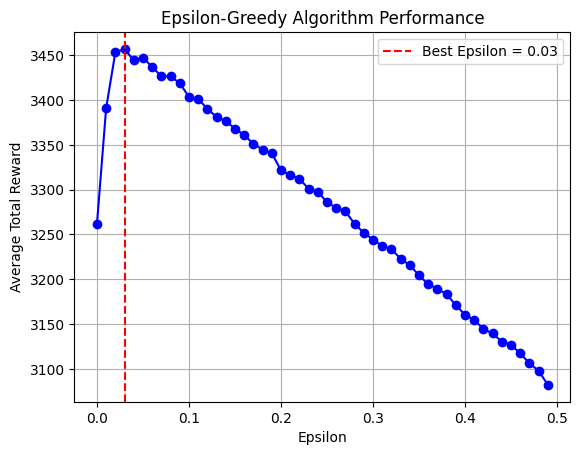
\includegraphics[width=\textwidth]{pics/greedy.png}
        \caption{\(\varepsilon\)-Greedy Results}
        \label{fig:epsilon_greedy}
    \end{subfigure}
    \hfill
    \begin{subfigure}[b]{0.45\textwidth}
        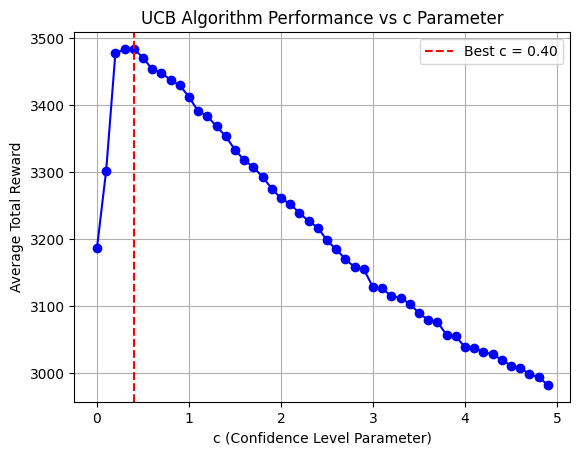
\includegraphics[width=\textwidth]{pics/ucb.png}
        \caption{UCB Results}
        \label{fig:ucb}
    \end{subfigure}
    \caption{Algorithm Performance Analysis}
    \label{fig:results}
\end{figure}

But even with the optimized parameters, the gap of the first two algorithms ($42.98$ and $16.10$ respectively) is still larger than \textbf{Thompson Sampling}, which has the smallest gap of $7.59$. Therefore, the \textbf{Thompson Sampling} algorithm is the best-performing algorithm in this scenario.


\subsubsection*{Parameter Impact Analysis}
\begin{enumerate}[1.]
\item \(\varepsilon\)-Greedy Algorithm

The \(\varepsilon\)-Greedy algorithm explores with probability \(\varepsilon\) and exploits with probability \(1 - \varepsilon\). The parameter \(\varepsilon\) controls the level of exploration versus exploitation.
\begin{itemize}
    \item \textbf{Low \(\varepsilon\) :}
    \begin{itemize}
        \item Pros: Prefer exploitation to exploration, leading to higher rewards when the current best action is optimal.
        \item Cons: Limited exploration may prevent discovery of better actions, especially in complex environments.
    \end{itemize}
    
    \item \textbf{High \(\varepsilon\) (e.g., \(\varepsilon = 0.5\)):}
    \begin{itemize}
        \item Pros: Increased exploration, potentially leading to the discovery of optimal actions.
        \item Cons: Excessive exploration dilutes the focus on known good actions, potentially lowering overall rewards.
    \end{itemize}
    
    \item \textbf{Optimal \(\varepsilon\):} Based on experiments, we find that \(\varepsilon = 0.03\) yields the highest average reward of 3457.02, indicating a good balance between exploration and exploitation. And when \(\varepsilon > 0.03\), the average reward decreases as the $\varepsilon$ (exploration) increases.
\end{itemize}

\item Upper Confidence Bound (UCB)

The UCB formula consists of two terms:

\begin{itemize}
    \item \textbf{Exploitation (\(\hat{\theta}(j)\)):} This term represents the current mean reward of action \(j\), which is used to exploit the known best action. The algorithm favors actions with a higher expected reward, leading to exploitation.
    
    \item \textbf{Exploration (\(c \cdot \sqrt{\frac{2 \ln(t)}{\text{count}(j)}}\)):} This term encourages exploration by adding a bonus to actions that have been chosen fewer times. The bonus is larger for actions that are less tested, which helps to balance exploration with the exploitation of known rewards. The parameter \(c\) controls the size of the exploration term. A higher \(c\) increases exploration, and a smaller \(c\) favors exploitation.
\end{itemize}
So the parameter \(c\) controls the trade-off between exploration and exploitation in the UCB algorithm, which is discussed as follows:
\begin{itemize}
    \item \textbf{Low \(c\):}
    \begin{itemize}
        \item Pros: Promotes exploitation as the confidence bounds become tighter.
        \item Cons: Reduced exploration can prevent the algorithm from discovering better actions.
    \end{itemize}
    
    \item \textbf{High \(c\):}
    \begin{itemize}
        \item Pros: Increases exploration by enlarging the confidence bounds, particularly for arms that have been pulled fewer times.
        \item Cons: Excessive exploration can reduce the focus on exploitation, potentially leading to suboptimal rewards.
    \end{itemize}
    
    \item \textbf{Optimal \(c\):} In our experiments, \(c = 0.40\) provides the best performance, yielding a maximum reward of 3483.90. And when \(c > 0.40\), the average reward decreases as the \(c\) (exploration) increases.
\end{itemize}

\item Thompson Sampling

The Thompson Sampling algorithm is a Bayesian method that uses prior and posterior beliefs to update the probability distribution for each action's reward. It assumes a Beta distribution as the prior for the reward probability of each arm, and updates the parameters \(\alpha_j\) and \(\beta_j\) based on the observed outcomes.

  \textbf{Prior Belief:}
    \begin{itemize}
        \item \(\alpha_j\) and \(\beta_j\) represent our prior belief about the reward distribution for action \(j\).
        \item For example, \(\alpha_j = 1\) and \(\beta_j = 1\) implies that we expect the reward probability for action \(j\) to be 50\%, but we have low confidence in this belief (uniform distribution).
        \item A higher value of \(\alpha_j\) relative to \(\beta_j\) means that we believe the reward probability for action \(j\) is higher, whereas a lower value of \(\alpha_j\) relative to \(\beta_j\) suggests that we believe the reward probability is lower.
    \end{itemize}

  \textbf{Effect of \(\alpha_j\) and \(\beta_j\):}
    \begin{itemize}
        \item \(\alpha_j\) and \(\beta_j\) are updated after each trial, based on whether the reward for action \(j\) was successful or not.
        \item When \(\alpha_j\) is large and \(\beta_j\) is small (e.g., \(\alpha_j = 2000\), \(\beta_j = 8000\)), we have a strong belief that the probability of a reward is low (20\%), and the algorithm exploits this information.
        \item When both \(\alpha_j\) and \(\beta_j\) are small (e.g., \(\alpha_j = 1\), \(\beta_j = 1\)), there is high uncertainty about the reward distribution, encouraging more exploration of different actions.
    \end{itemize}

\end{enumerate}


\newpage
\subsection{Problem 5}
The exploration-exploitation trade-off is a central challenge in decision-making processes, particularly in bandit algorithms. It arises when an agent, tasked with maximizing some reward, must decide how much to explore new options (i.e., gather more data) versus exploiting known, high-reward options based on the information it already has.

\textbf{Exploration} involves trying out different actions to gather more information about their outcomes, even if these actions might not seem optimal in the short term. This is essential in the early stages when little is known about the environment.

\textbf{Exploitation} involves choosing the option that has historically provided the highest reward, based on the information the agent has collected. The idea is to maximize immediate rewards using known information.

The trade-off occurs because if the agent always explores, it might fail to capitalize on known high-reward actions. On the other hand, if it always exploits, it risks missing potentially better actions that could be discovered through exploration. Thus, the challenge is in balancing exploration and exploitation over time to optimize overall rewards.

\subsubsection*{Algorithms for Addressing the Exploration-Exploitation Trade-off}
\begin{enumerate}[1.]
  \item Epsilon-Greedy Algorithm:
  The epsilon-greedy algorithm provides a simple way to balance exploration and exploitation:
  \begin{itemize}
    \item With probability $\varepsilon$, the agent explores (chooses a random action).
    \item With probability $1 - \varepsilon$, the agent exploits (chooses the action that has provided the highest reward so far).
  \end{itemize}
  The parameter $\varepsilon$ controls the balance between exploration and exploitation. If $\varepsilon$ is high, the agent explores more, while if it is low, it exploits more.

  \textbf{Challenge:} The main limitation of the epsilon-greedy approach is that it uses a fixed $\varepsilon$ throughout the process. Over time, an agent might need to explore less and exploit more, but a fixed $\varepsilon$ might not reflect this need. Adjusting $\varepsilon$ over time (e.g., decreasing $\varepsilon$ as the agent learns more) can improve performance, where more exploration is done at the beginning and exploitation increases as certainty builds.
  
  \item Upper Confidence Bound (UCB) Algorithm:
  The UCB algorithm is based on the idea of balancing exploration and exploitation by considering both the average reward of each action and the uncertainty in the estimate of that reward:
  \begin{itemize}
    \item For each arm (action), UCB calculates an upper bound on the potential reward based on how many times the arm has been selected and the variance in its reward.
    \item The agent then selects the arm with the highest upper bound, balancing the need to exploit the best-known action and explore those with high uncertainty.
  \end{itemize}
  The UCB algorithm relies on Hoeffding's inequality to estimate the confidence intervals for each arm's expected reward. The algorithm rewards actions with high uncertainty to ensure that they are explored adequately while still exploiting actions with the highest observed reward.
  
  \textbf{Advantage:} As time progresses, the UCB algorithm places more weight on exploitation as uncertainty decreases, gradually refining the agent's knowledge. It inherently balances exploration and exploitation without requiring manual adjustment of the exploration rate.

  \item Thompson Sampling Algorithm
  Thompson Sampling takes a probabilistic approach to the exploration-exploitation trade-off, using Bayesian inference:
  \begin{itemize}
    \item Each arm is modeled by a Beta distribution (since Beta is the conjugate prior for Bernoulli/binomial likelihood), and the parameters of this distribution represent the belief about the arm's reward.
    \item The agent samples from the Beta distributions and selects the arm with the highest sampled reward.
    \item After each trial, the agent updates the Beta distribution based on the observed reward, refining its belief about the arm's expected reward.
  \end{itemize}
  The agent uses prior knowledge (if available) and updates its beliefs about the rewards using the observed data. In this way, the exploration-exploitation trade-off is handled naturally by the sampling process: arms with higher uncertainty (higher variance in their Beta distribution) are explored more, while arms with lower uncertainty are exploited.
  
  \textbf{Advantage:} Thompson Sampling is highly effective and tends to outperform epsilon-greedy and UCB in many scenarios, particularly when the true reward distributions are well-modeled by Beta distributions. The algorithm's probabilistic nature makes it flexible and robust across different situations.
\end{enumerate}
Ultimately, the exploration-exploitation trade-off is about finding a strategy that maximizes cumulative rewards over time. While epsilon-greedy is easy to implement and useful for simpler environments, UCB and Thompson Sampling are more sophisticated and provide better performance in many complex scenarios, especially when the agent's knowledge about the environment is continuously evolving.

\newpage
\subsection{Problem 6}
\subsubsection*{Problem Settings (Dependent Case)}
We examine a multi-armed bandit problem featuring three interdependent arms. This scenario introduces a dependency between the arms, which is set as follows:

After each arm pull, the probabilities are adjusted based on the outcome:
\begin{itemize}
    \item \textbf{If a reward is obtained} from pulling arm \(j\) (\(\text{reward} = 1\)):
    \begin{align*}
        \theta_j &\leftarrow \max(\theta_j - p, 0) \\
        \theta_k &\leftarrow \min(\theta_k + \frac{p}{2}, 1) \quad \forall k \neq j
    \end{align*}
    
    \item \textbf{If no reward is obtained} from pulling arm \(j\) (\(\text{reward} = 0\)):
    \begin{align*}
        \theta_j &\leftarrow \min(\theta_j + p, 1) \\
        \theta_k &\leftarrow \max(\theta_k - \frac{p}{2}, 0) \quad \forall k \neq j
    \end{align*}
\end{itemize}
These adjustments ensure that the reward probabilities remain within the valid range \([0, 1]\).

\paragraph{Experimental Setup}
To evaluate the performance of the algorithms under the independent settings, the following parameters are used:

\begin{itemize}
    \item \textbf{Number of Time Steps} (\( N \)): 5000.
    \item \textbf{Number of Trials} (\( \text{repeat\_time} \)): 100.
    \item \textbf{Adjustment Parameter} (\( p \)): 0.005.
\end{itemize}

\paragraph{Objective}
The primary goal is to determine the optimal algorithmic parameters that maximize the average total reward over \( N \) time steps across multiple trials.

\subsubsection*{Algorithm Design}
For the dependent case, we test the three original algorithms on dependent arms. Then, we implement a new algorithm, \texttt{Dependency-Aware Thompson Sampling} (DATS), which adapts the Thompson Sampling algorithm to account for the interdependence between arms to obtain a better result.

\begin{description}
\item[Algorithm Description:] The Dependency-Aware Thompson Sampling with Dynamic Environment Updates algorithm is designed to handle non-stationary environments where arm probabilities change over time and there are potential dependencies between arms. The algorithm operates as follows:
\begin{enumerate}
    \item \textbf{Initialization:} 
    \begin{itemize}
        \item Initialize probabilities ($\theta$) for each arm.
        \item Set initial Beta distribution parameters ($\alpha$ and $\beta$) for each arm.
        \item Define parameters: $N$ (number of iterations), $p$ (probability update rate), $\epsilon$ (exploration rate), $\gamma$ (dependency factor).
    \end{itemize}
    
    \item \textbf{Arm Selection:} For each iteration $t$ from 1 to $N$:
    \begin{itemize}
        \item With probability $\epsilon$, explore by choosing a random arm.
        \item Otherwise (probability $1-\epsilon$), exploit using Thompson Sampling:
        \begin{itemize}
            \item For each arm $i$, sample a value from Beta($\alpha_i$, $\beta_i$).
            \item Choose the arm with the highest sampled value.
        \end{itemize}
    \end{itemize}
    
    \item \textbf{Reward Observation:} 
    \begin{itemize}
        \item Observe a reward (0 or 1) based on the current probability of the chosen arm.
        \item Add the reward to the total reward.
    \end{itemize}
    
    \item \textbf{Beta Distribution Update:} 
    \begin{itemize}
        \item If reward = 1:
        \begin{itemize}
            \item Increment $\alpha$ of the chosen arm by 1.
            \item If $\gamma > 0$, increment $\alpha$ of all other arms by $\gamma$.
        \end{itemize}
        \item If reward = 0:
        \begin{itemize}
            \item Increment $\beta$ of the chosen arm by 1.
            \item If $\gamma > 0$, increment $\beta$ of all other arms by $\gamma$.
        \end{itemize}
    \end{itemize}
    
    \item \textbf{Return:} Total accumulated reward over all iterations.
\end{enumerate}


\item[Key Features:] This approach combines several strategies to handle the challenges of a non-stationary, dependent arm environment:

\begin{itemize}
    \item The $\epsilon$-greedy method ensures continued exploration, which is crucial for detecting changes in the environment.
    \item Thompson Sampling provides a balance between exploration and exploitation based on the current beliefs about arm probabilities.
\end{itemize}

\end{description}
\begin{algorithm}[H]
\caption{Dependency-Aware Thompson Sampling}
\label{alg:DA-TS}
\begin{algorithmic}[1]
\Ensure Total cumulative reward $\text{total\_reward}$
\State $\alpha \gets \alpha_{\text{init}}$
\State $\beta \gets \beta_{\text{init}}$
\State $K \gets \text{length}(\alpha)$
\State $\theta_{\text{current}} \gets \theta$
\State $\text{total\_reward} \gets 0$
\For{$t \gets 1$ to $N$}
    \If{$\text{Uniform}(0,1) < \epsilon$}
        \State $\text{chosen\_arm} \gets \text{Random}(\{1,\ldots,K\})$
    \Else
        \For{$i \gets 1$ to $K$}
            \State $\text{samples}[i] \gets \text{Beta}(\alpha[i], \beta[i])$
        \EndFor
        \State $\text{chosen\_arm} \gets \arg\max(\text{samples})$
    \EndIf
    \State $\text{reward} \gets \mathbb{1}[\text{Uniform}(0,1) < \theta_{\text{current}}[\text{chosen\_arm}]]$
    \State $\text{total\_reward} \gets \text{total\_reward} + \text{reward}$
    \If{$\text{reward} = 1$}
        \State $\alpha[\text{chosen\_arm}] \gets \alpha[\text{chosen\_arm}] + 1$
        \For{$\text{other\_arm} \in \{1,\ldots,K\} \setminus \{\text{chosen\_arm}\}$}
            \State $\alpha[\text{other\_arm}] \gets \alpha[\text{other\_arm}] + \gamma$
        \EndFor
    \Else
        \State $\beta[\text{chosen\_arm}] \gets \beta[\text{chosen\_arm}] + 1$
        \For{$\text{other\_arm} \in \{1,\ldots,K\} \setminus \{\text{chosen\_arm}\}$}
            \State $\beta[\text{other\_arm}] \gets \beta[\text{other\_arm}] + \gamma$
        \EndFor
    \EndIf
\EndFor
\State \Return $\text{total\_reward}$
\end{algorithmic}
\end{algorithm}



\newpage
\subsubsection*{Results and Analysis}
\setstretch{1}
\begin{figure}[H]
    \centering
    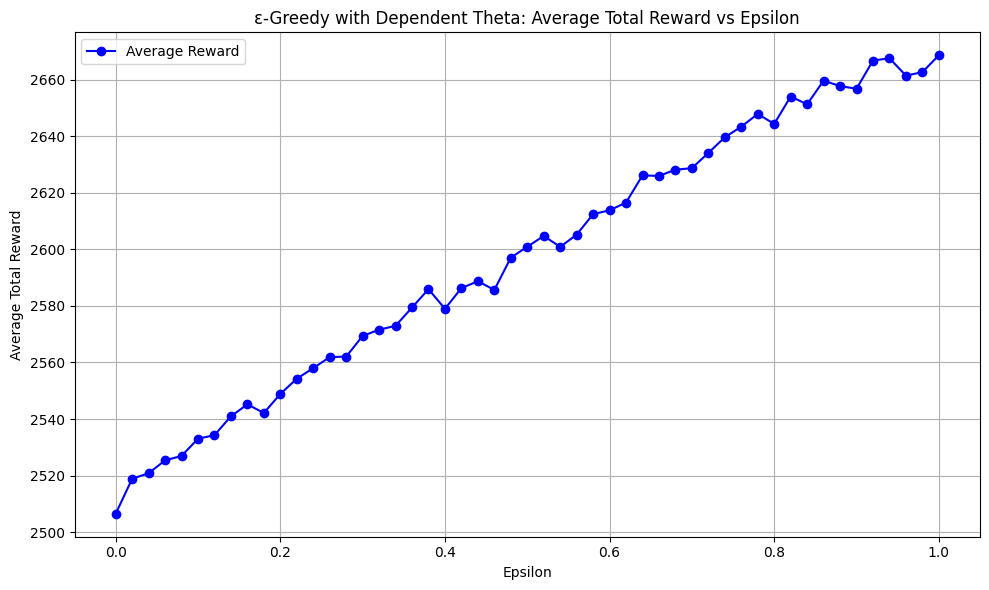
\includegraphics[width=0.8\textwidth]{pics/greedy_dependence.png}
    \caption{Dependent \(\varepsilon\)-Greedy Performance}
    \label{fig:greedy_dependence}
\end{figure}

\begin{figure}[H]
    \centering
    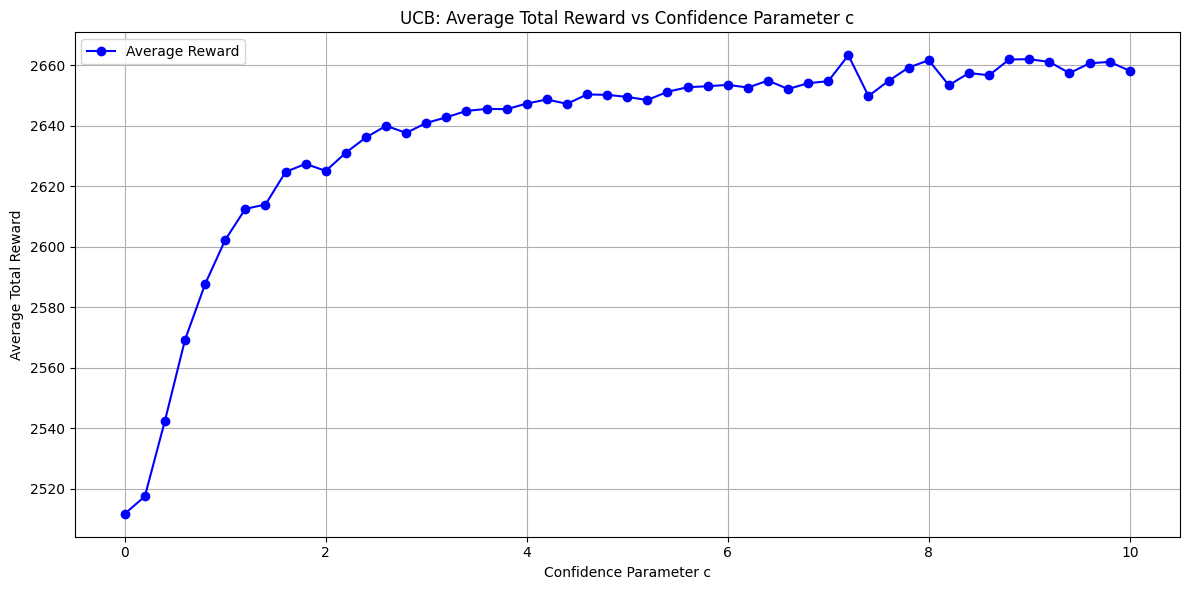
\includegraphics[width=0.8\textwidth]{pics/ucb_dependence.png}
    \caption{Dependent UCB Performance}
    \label{fig:ucb_dependence}
\end{figure}

\begin{figure}[H]
    \centering
    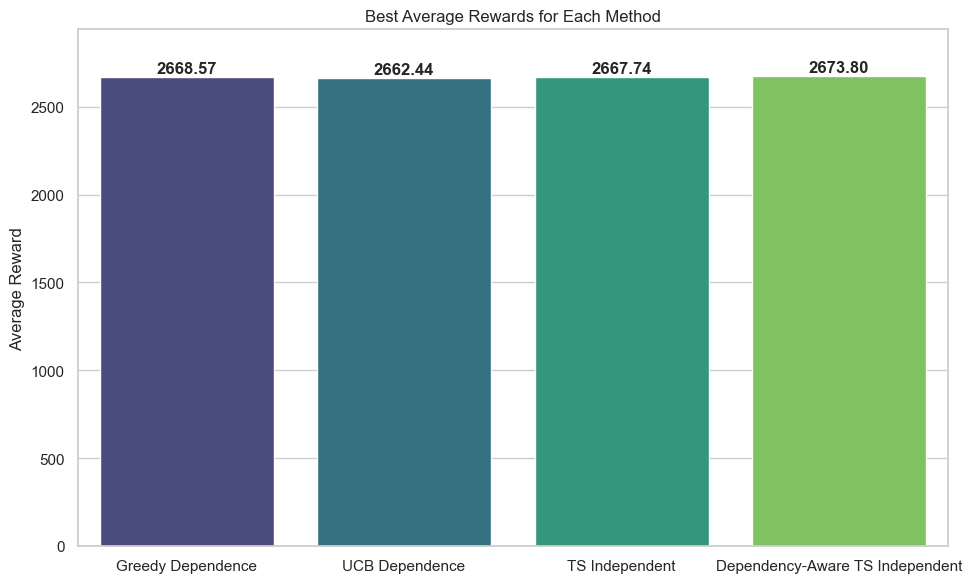
\includegraphics[width=0.8\textwidth]{pics/best_average_rewards.png}    
    \caption{Comparison of TS and DATS with Different Alpha1}
    \label{fig:best_average_rewards}
\end{figure}

\begin{figure}[H]
    \centering
    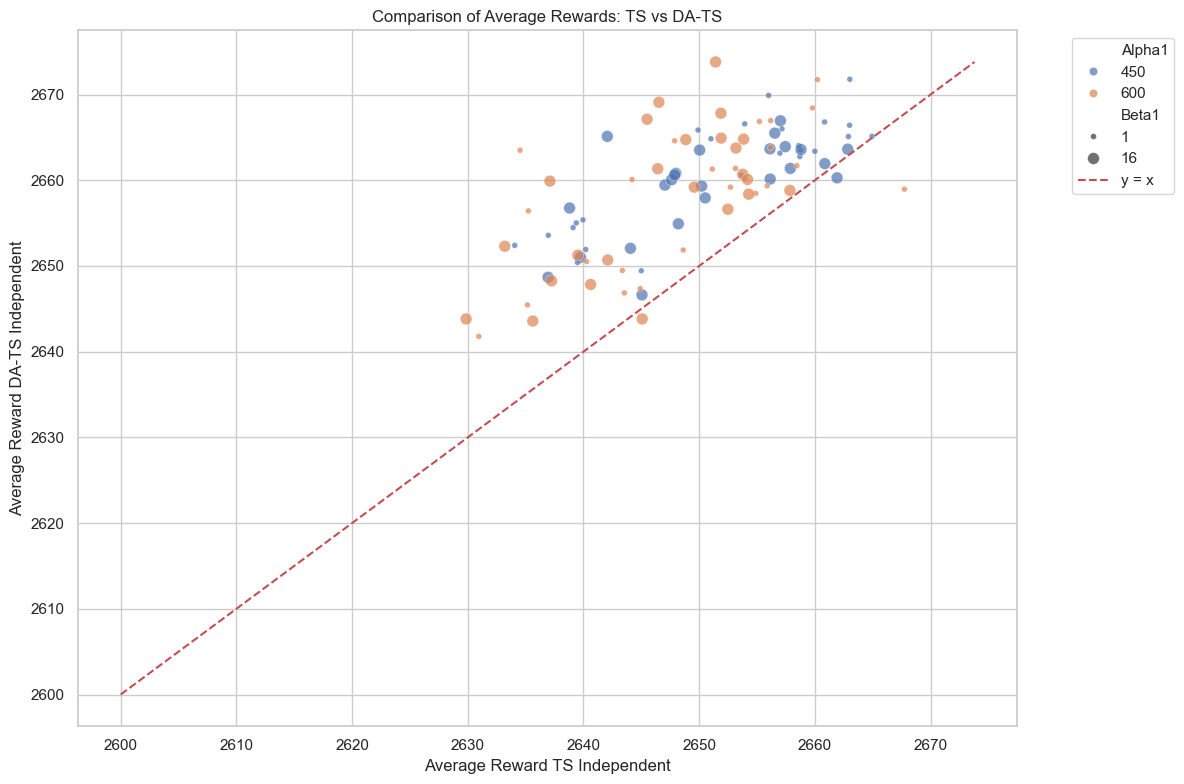
\includegraphics[width=0.8\textwidth]{pics/comparison_scatter.png}
    \caption{Comparison of TS and DATS}
    \label{fig:comparison_scatter}
\end{figure}

\newpage
By experimenting, we receive the following results:
\begin{table}[H]
    \centering
    \begin{tabularx}{\textwidth}{|X|X|c|}
        \hline
        \textbf{Algorithm} & \textbf{Best Parameters} & \textbf{Maximum Reward} \\
        \hline
        \(\varepsilon\)-Greedy & \(\varepsilon = 1.00\) & 2668.57 \\
        \hline
        UCB & \(c = 8.60\) & 2662.44 \\
        \hline
        Thompson Sampling & \(\begin{array}{l}
            \alpha = [600, 300, 450] \\
            \beta = [1, 1, 31]
        \end{array}\) & 2667.74 \\
        \hline
        Dependency-Aware TS & \(\begin{array}{l}
            \alpha = [600, 450, 450] \\
            \beta = [16, 16, 31] \\
            \epsilon = 0.001 \\
            \gamma = 10^{-6}
        \end{array}\) & 2673.80 \\
        \hline
    \end{tabularx}
    \caption{Performance Comparison of Bandit Algorithms}
    \label{tab:algorithm_comparison}
\end{table}

\setstretch{1.1}

The experimental results presented in Figures \ref{fig:greedy_dependence}, \ref{fig:ucb_dependence}, \ref{fig:best_average_rewards}, \ref{fig:comparison_scatter}, and Table \ref{tab:algorithm_comparison} provide compelling evidence for the superiority of our proposed Dependency-Aware Thompson Sampling (DATS) algorithm over the other four methods examined: Greedy Dependence, UCB Dependence, and TS Independent.

\begin{enumerate}
    \item \textbf{Superior Performance:} As shown in Figure \ref{fig:best_average_rewards} and Table \ref{tab:algorithm_comparison}, DATS achieves the highest average reward (2673.80) among all methods tested. This outperforms Greedy Dependence (2668.57), UCB Dependence (2662.44), and TS Independent (2667.74), demonstrating DATS's ability to make more informed decisions in multi-armed bandit problems with dependent arms.

    \item \textbf{Consistent Outperformance:} The scatter plot in Figure \ref{fig:comparison_scatter} illustrates that DATS consistently outperforms the TS Independent method across various parameter settings. The majority of points lie above the $y=x$ line, indicating that DATS yields higher average rewards in most scenarios.

    \item \textbf{Robustness to Hyperparameters:} Unlike the Greedy Dependence (Figure \ref{fig:greedy_dependence}) and UCB Dependence (Figure \ref{fig:ucb_dependence}) methods, which show high sensitivity to their respective hyperparameters ($\epsilon$ and confidence parameter $c$), DATS demonstrates more stable performance across different settings. This robustness is a crucial advantage in real-world applications where optimal hyperparameter tuning may be challenging.
\end{enumerate}

\newpage
\section{Part II: Bayesian Bandit Algorithms}
\subsection{Problem 1}

\end{document}